\section*{Aufgabe 1}
\subsection*{a)}
Die Differentialgleichung (DGL) 
\begin{equation}
    \ddot{x} + \alpha \dot{x} + x = 0
\end{equation}
beschreibt einen harmonischen Oszillator mit Dämpfung $\alpha$.
Gelöst wird die DGL über den Ansatz 
\begin{equation}
    x(t) = e^{\lambda t}
\end{equation}
und führt zur Lösung 
\begin{equation}
    x(t) = c_1 e^{\lambda_1 t} + c_2 e^{\lambda_2 t}
\end{equation}
mit 
\begin{equation}
    \lambda_{1,2} = - \frac{\alpha}{2} \pm \sqrt{ \frac{\alpha^2}{4} -1 }.
\end{equation}
Es ergeben sich folgende Fälle:
\begin{enumerate}
    \item $\alpha = 0$ : Harmonischer Oszialltor (Abbildung \ref{fig:harmonisch}).
    \item $\frac{\alpha^2}{4} > \omega^2 = 1$: Kriechfall (Abbildung \ref{fig:Kriech}).
    \item $\frac{\alpha^2}{4} = \omega^2 = 1$: Aperiodischer Grenzfall (Abbildung \ref{fig:Aperiodisch}).
    \item $\frac{\alpha^2}{4} < \omega^2 = 1$: Gedämpfte Schwingung (Abbildung \ref{fig:gedämpft}).
\end{enumerate}
Zur Darstellung des Oszillationsverhaltens wurden dabei 3D-Scatter-Plots gewählt.
\begin{figure}
  \centering
  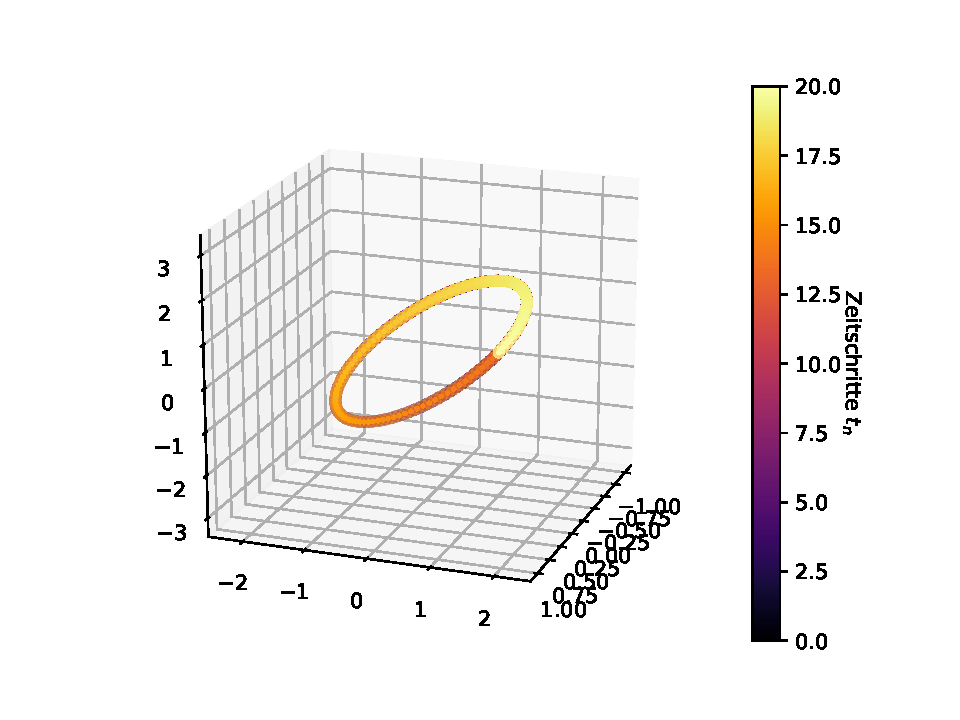
\includegraphics[scale=0.7]{A2/build/Plots/aufg1_a1.pdf}
  \caption{Trajektorie eines Harmonischen Oszilators ($\alpha = 0$).}
  \label{fig:harmonisch}
\end{figure}

\begin{figure}[H]
  \centering
  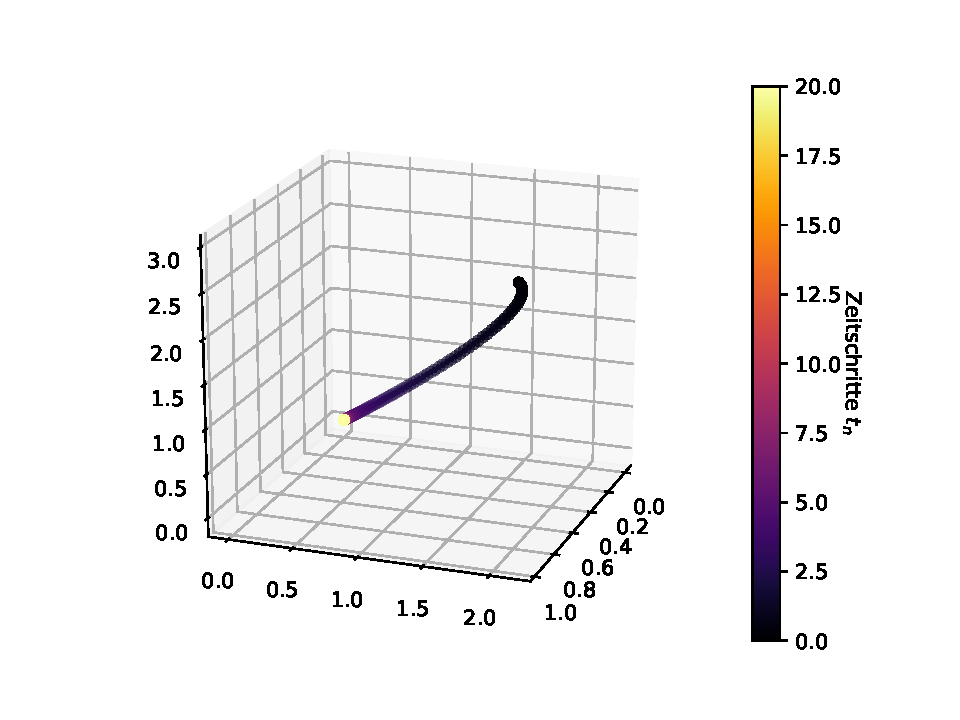
\includegraphics[scale=0.7]{A2/build/Plots/aufg1_a2.pdf}
  \caption{Trajektorie den aperiodischen Grenzfall für $\alpha = 2$.}
  \label{fig:Aperiodisch}
\end{figure}

\begin{figure}[H]
  \centering
  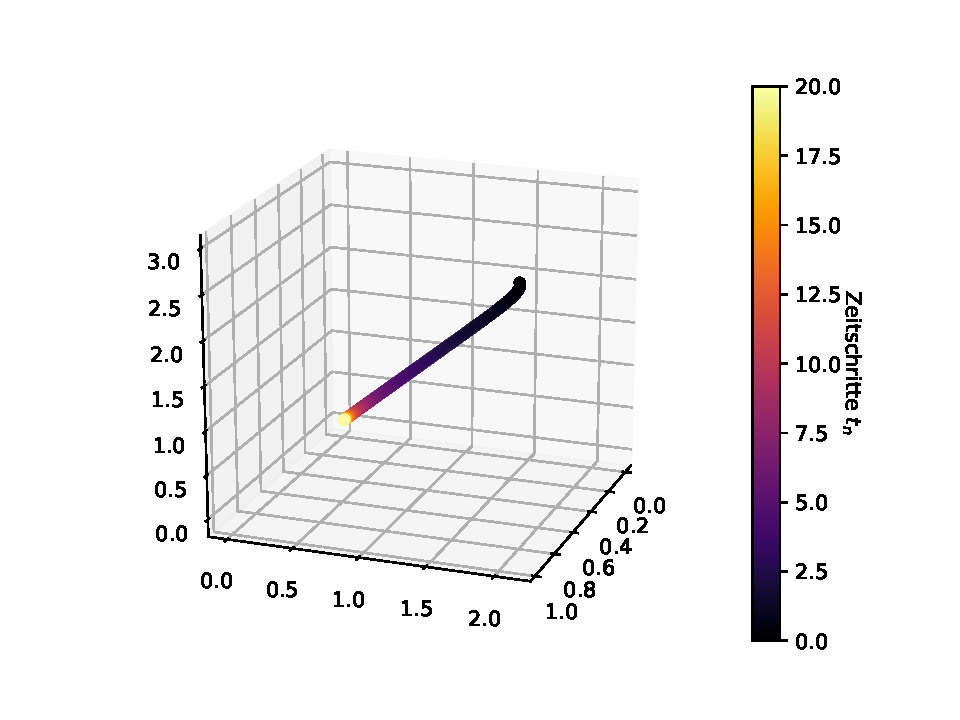
\includegraphics[scale=0.7]{A2/build/Plots/aufg1_a3.pdf}
  \caption{Trajektorie den Kriechfall für $\alpha = 4$.}
  \label{fig:Kriech}
\end{figure}

\begin{figure}[H]
  \centering
  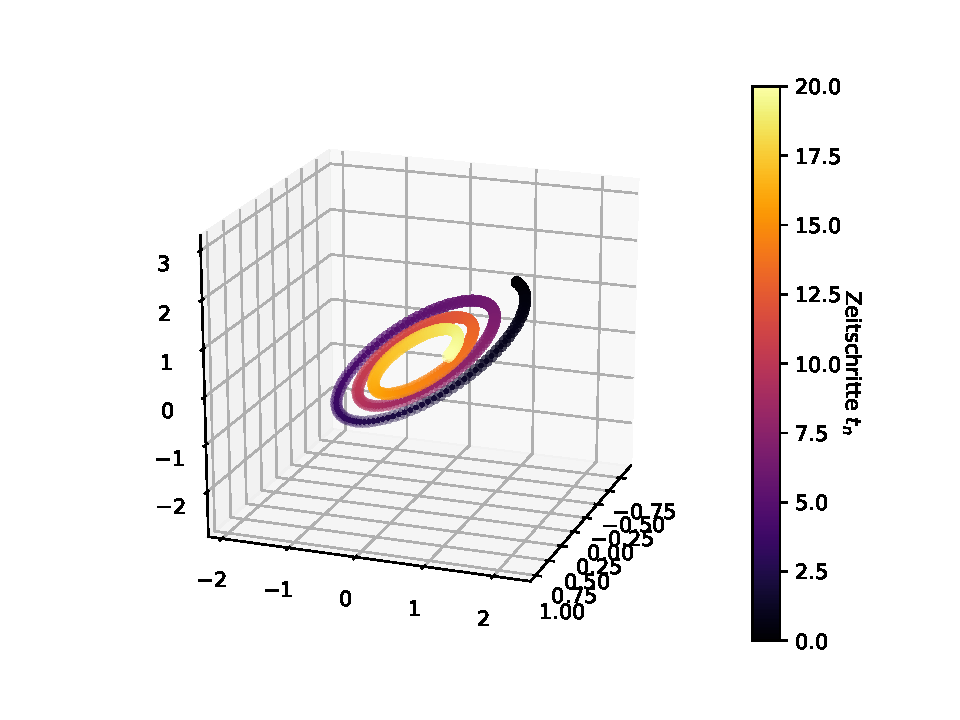
\includegraphics[scale=0.7]{A2/build/Plots/aufg1_a4.pdf}
  \caption{Trajektorie die gedämpfte Schwingung $\alpha = 0.1$.}
  \label{fig:gedämpft}
\end{figure}

\subsection*{b)}
Die Gesamtenergie $E_{Ges} = E_{kin} + E_{pot}$ ist für einen harmoschen Oszialltor erhalten. Da wir hier jedoch einen Oszialltor mit Dämpfung betrachten, geht durch die Dämpfung imemr ein Teil der Gesamtenergie verloren.
In Abbildung \ref{fig:energie} ist die Gesamtenergie pro Zeit dargestellt.

\begin{figure}
  \centering
  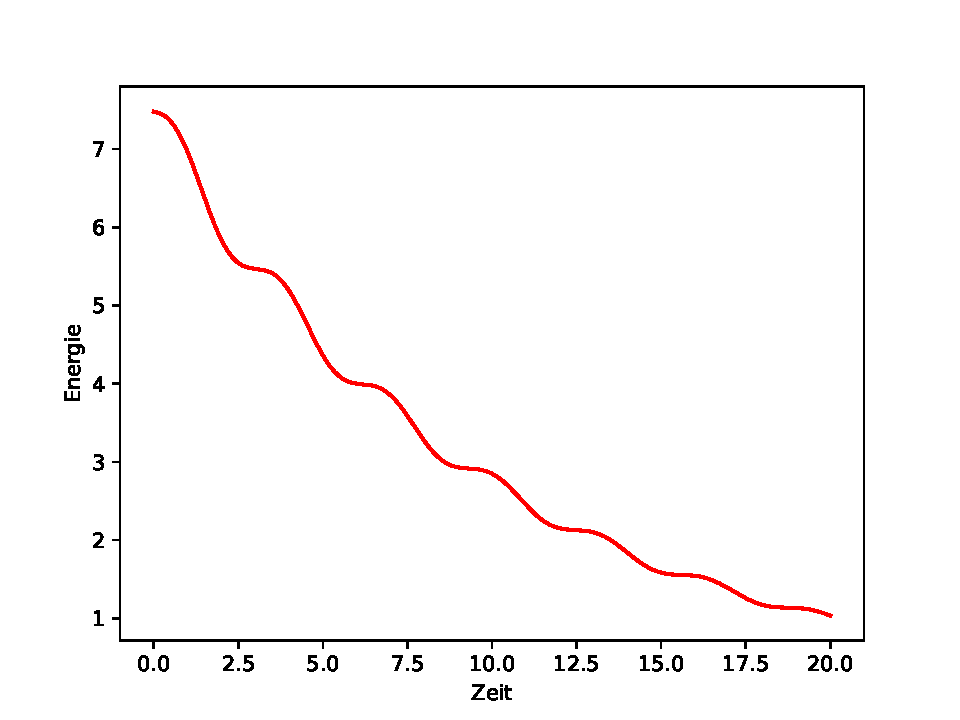
\includegraphics[scale=0.7]{A2/build/Plots/Energie.pdf}
  \caption{Verlauf der Gesamtenergie für ein harmonisches Potential.}
  \label{fig:energie}
\end{figure}

%\subsection*{c)}
%
%
%Zeit Adams: 0.003271.sec
%Zeit Runge: 0.003343.sec
%Zeit Adams 2 : 0.0042.sec
%Zeit Runge 2 : 0.003325.sec
%
%Für ein Zeitintervall von $1000$ und eine Schrittweite von $30000$ ergibt sich für das Adams-Bashforth-Verfahren eine Laufzeit %von \SI{0.519792}{\s}, während sich für das Runge-Kutta-Verfahren eine Zeit von \SI{0.543176}{\s} ergibt.
%Somit ist das Adams-Bashforth-Verfahren etwas schneller. 
